\paragraph{Sơ đồ tuần tự luồng Tạo mới gói thuê bao VIP}

Luồng nghiệp vụ này mô tả
quy trình Quản trị viên (Admin)
thực hiện tạo mới một gói thuê bao VIP (Plan)
trong hệ thống.

\begin{figure}[H]
\centering
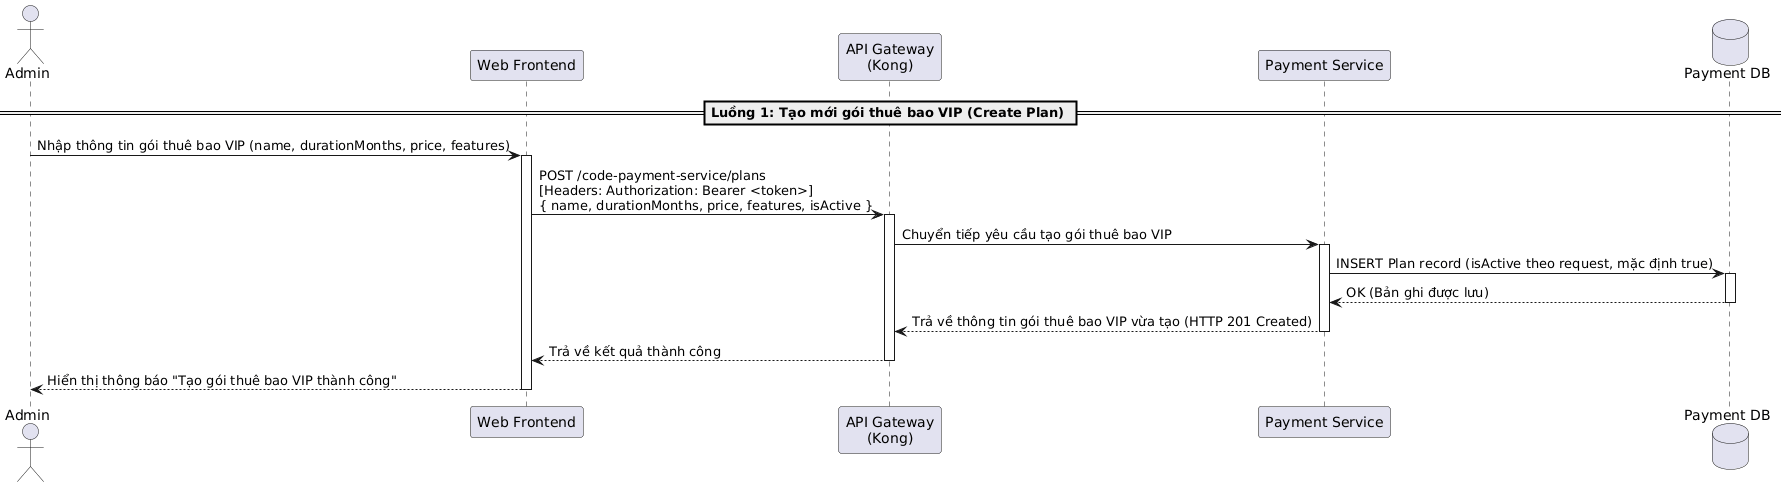
\includegraphics[scale = 0.2]{contents/Sequence/UML-Sequence-AdminCreateVipPlan.png}
\caption{Sơ đồ tuần tự luồng Tạo mới gói thuê bao VIP}
\end{figure}

\subparagraph{Các thành phần tham gia}

\begin{table}[H]
\centering
\renewcommand{\arraystretch}{1.3}

\begin{tabular}{|l|l|p{5cm}|}
\hline
\textbf{Thành phần} & \textbf{Phân loại} & \textbf{Vai trò trong hệ thống} \\ \hline
Admin & Actor & Quản trị viên thực hiện quản lý danh mục gói thuê bao VIP. \\ \hline
Web Frontend & Component & Giao diện web Next.js. \\ \hline %%%% Component & Giao diện Admin hiển thị form tạo mới gói thuê bao VIP. \\ \hline
API Gateway (Kong) & Component & Cổng API chuyển tiếp các yêu cầu API. \\ \hline %%%% Component & Định tuyến yêu cầu an toàn đến Payment Service và kiểm tra quyền Admin. \\ \hline
Payment Service & Microservice & Tiếp nhận yêu cầu, xử lý và tạo gói thuê bao VIP. \\ \hline
Payment Database & Database & Lưu trữ thông tin chi tiết về các gói thuê bao VIP (Plan). \\ \hline
\end{tabular}
\caption{Các thành phần tham gia luồng Tạo mới gói thuê bao VIP}
\end{table}

\subparagraph{Mô tả tổng quan}

\begin{itemize}
\item \textbf{Yêu cầu tạo mới:}
Quản trị viên điền thông tin gói thuê bao VIP
mới.
\item \textbf{Gửi yêu cầu:}
Giao diện gửi yêu cầu tạo gói thuê bao VIP mới
kèm mã xác thực qua cổng API.
\item \textbf{Xử lý và lưu trữ:}
Dịch vụ thanh toán tiếp nhận yêu cầu,
ghi nhận thông tin gói thuê bao VIP mới vào
CSDL ở trạng thái đang hoạt động
và phản hồi thông tin gói vừa tạo về giao diện cho quản trị viên.
\end{itemize}
